\documentclass[tikz,border=5pt]{standalone}
\usetikzlibrary{arrows.meta}
\usetikzlibrary{backgrounds}
\usetikzlibrary{calc}
\newcommand*{\TickSize}{2pt}%

\begin{document}
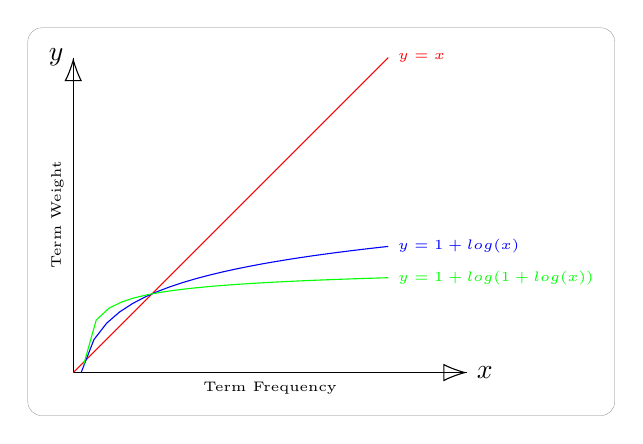
\begin{tikzpicture}
	[framed,background rectangle/.style={ultra thin, rounded corners=5pt, draw=gray}];

	%Axis
	\coordinate (x) at (5,0);
	\coordinate (y) at (0,4);
	\coordinate (o) at (0,0);
	\draw[-{Latex[length=3mm,open]}] (o)--(x) node[right]{$x$};
	\draw (o) -- (x) node [midway, below, sloped] (textX) {\tiny Term Frequency};
	\draw[-{Latex[length=3mm,open]}] (o)--(y) node[left]{$y$};
	\draw (o) -- (y) node [midway, above, sloped] (textY) {\tiny Term Weight};

	%coordinate
	\draw [draw=red]plot [domain=0:4] (\x,\x) node[anchor=west,red]{\tiny $y=x$};
	\draw [draw=blue] plot [domain=0.1:4] (\x,{1+log10(+\x)}) node[anchor=west,blue]{\tiny$y=1+log(x)$} ;
	\draw [draw=green] plot [domain=0.13:4] (\x,{1+log10(1+log10(\x))}) node[anchor=west,green]{\tiny $y=1+log(1+log(x))$};
\end{tikzpicture}
\end{document}